%% start of file `template.tex'.
%% Copyright 2006-2013 Xavier Danaux (xdanaux@gmail.com).
%
% This work may be distributed and/or modified under the
% conditions of the LaTeX Project Public License version 1.3c,
% available at http://www.latex-project.org/lppl/.


\documentclass[11pt,a4paper,roman]{moderncv}        % possible options include font size ('10pt', '11pt' and '12pt'), paper size ('a4paper', 'letterpaper', 'a5paper', 'legalpaper', 'executivepaper' and 'landscape') and font family ('sans' and 'roman')

%\moderncvstyle{perso}
% modern themes
\moderncvstyle{banking}                            
%\moderncvstyle{casual}                            
% style options are 'casual' (default), 'classic', 'oldstyle' and 'banking'
\moderncvcolor{orange}                                % color options 'blue' (default), 'orange', 'green', 'red', 'purple', 'grey' and 'black'
%\renewcommand{\familydefault}{\sfdefault}         % to set the default font; use '\sfdefault' for the default sans serif font, '\rmdefault' for the default roman one, or any tex font name
%\nopagenumbers{}                                  % uncomment to suppress automatic page numbering for CVs longer than one page

% character encoding
\usepackage[utf8]{inputenc}                       % if you are not using xelatex ou lualatex, replace by the encoding you are using
%\usepackage{CJKutf8}                              % if you need to use CJK to typeset your resume in Chinese, Japanese or Korean
\usepackage{textgreek}
\usepackage{dictsym}
% adjust the page margins
\usepackage[scale=0.75]{geometry}
%\setlength{\hintscolumnwidth}{3cm}                % if you want to change the width of the column with the dates
%\setlength{\makecvtitlenamewidth}{10cm}           % for the 'classic' style, if you want to force the width allocated to your name and avoid line breaks. be careful though, the length is normally calculated to avoid any overlap with your personal info; use this at your own typographical risks...

%\usepackage{draftwatermark}
%\SetWatermarkText{DRAFT}
%\SetWatermarkScale{1}
\definecolor{fondentreprise}{rgb}{0.96, 0.94, 0.93}
%\definecolor{fondentreprise}{rgb}{0.95,0.55,0.15}% orange
\definecolor{amber}{rgb}{1.0, 0.75, 0.0}
%\usepackage{amssymb}
\usepackage{bbding}
\usepackage{import}
\usepackage{fancyhdr}
\usepackage{fontawesome}
%\usepackage[arrows]{boisik}
\pagestyle{fancy}
\renewcommand{\footrulewidth}{0.4pt}
%\fancyhead[LE,RO]{\slshape \rightmark}
\fancyfoot[L]{\tiny{git : \input{gitlog.tex}}}
%\newcommand{\myvspace}{\\\\[6pt]}
\newcommand{\myitem}[2]{\item{\textbf{#1} #2}\vspace{5pt}}
\newcommand{\myhr}{\noindent\hfill{\rule{4cm}{0.4pt}}\hfill}


%\newcommand\itemq{\item[\textbf{\textPsi}]}
%\newcommand\itemq{\item[\textbf{\dstechnical}]}
\newcommand\itemq{\item[\textbf{\Sparkle}]}

%\usepackage{marvosym}
\newcommand\itemformation{\item[\textbf{\dstechnical}]}
%\newcommand\itemskill[2]{\item[\textcolor{orange}{\small{\faHandORight}}]\underline{#1} : #2 \vspace{0.1cm}}
\newcommand\itemskill[2]{\item[]\underline{\textit{\textbf{#1}}} : #2 \vspace{0.1cm}}

\usepackage{allrunes}
\usepackage{epiolmec}
\usepackage{MnSymbol}
%\newcommand\itemexperience{\item[\textcolor{orange}{\AsteriskThinCenterOpen}]}
\newcommand\itemexperience{\item[]}

\newcommand\cventrylc[6]{
\fcolorbox{white}{fondentreprise}{\makebox[15.5cm]{\makebox [4cm][l]{
%\AsteriskThinCenterOpen\hspace*{0.2cm}
\textit{#1}}\makebox[11.5cm][r]{\textbf{#3} \textit{\small{(#4)}}}}}
\newline
\fcolorbox{white}{white}{\textbf{\textit{#2}}}
\newline
{#5}{#6}
%\myhr
\vspace{0.5cm}
}

\input{langue.tex}
%\newtoggle{anglais}
%\toggletrue{anglais}

% personal data
\name{Laurent}{Carrié}
\vspace{5pt}

%\title{Curriculum Vitae}                               % optional, remove / comment the line if not wanted

\address{Senior Software Architect}{}{}% optional, remove / comment the line if not wanted; the "postcode city" and and "country" arguments can be omitted or provided empty
\phone[mobile]{+33 (0)6 76 47 92 42}                   % optional, remove / comment the line if not wanted
%\phone[fixed]{01234 123456}                    % optional, remove / comment the line if not wanted
%\phone[fax]{+3~(456)~789~012}                      % optional, remove / comment the line if not wanted
\email{laurent.carrie@gmail.com}                               % optional, remove / comment the line if not wanted
%\homepage{www.myname.webs.com} 
\social[linkedin]{laurent-carrie}
% optional, remove / comment the line if not wanted
%\extrainfo{additional information}                 % optional, remove / comment the line if not wanted
\extrainfo{nationalité française}
%\photo[64pt][0.4pt]{id.jpg}                       % optional, remove / comment the line if not wanted; '64pt' is the height the picture must be resized to, 0.4pt is the thickness of the frame around it (put it to 0pt for no frame) and 'picture' is the name of the picture file
%\quote{Some quote}                                 % optional, remove / comment the line if not wanted

% to show numerical labels in the bibliography (default is to show no labels); only useful if you make citations in your resume
%\makeatletter
%\renewcommand*{\bibliographyitemlabel}{\@biblabel{\arabic{enumiv}}}
%\makeatother
%\renewcommand*{\bibliographyitemlabel}{[\arabic{enumiv}]}% CONSIDER REPLACING THE ABOVE BY THIS

% bibliography with mutiple entries
%\usepackage{multibib}
%\newcites{book,misc}{{Books},{Others}}

%\geometry{left=0.2cm, top=1.5cm, right=2cm, bottom=2cm, footskip=.5cm}
% Configure page margins with geometry


\input{watermark}

%----------------------------------------------------------------------------------
%            content
%----------------------------------------------------------------------------------

\usepackage{setspace}

%\patchcmd{\makehead}
  {\hfil}
  {\hspace*{0.15\textwidth}}
  {}
  {}
\patchcmd{\makehead}
  {\setlength{\makeheaddetailswidth}{0.8\textwidth}}
  {\setlength{\makeheaddetailswidth}{0.67\textwidth}}
  {}
  {}
\patchcmd{\makehead}
  {\\[2.5em]}
  {\hfil\raisebox{-.7cm}{\framebox{\includegraphics[width=\@photowidth]{\@photo}}}\\[2.5em]}
  {}
  {}
  
  
\begin{document}
%\begin{CJK*}{UTF8}{gbsn}                          % to typeset your resume in Chinese using CJK
%-----       resume       ---------------------------------------------------------
%\makecvtitle
%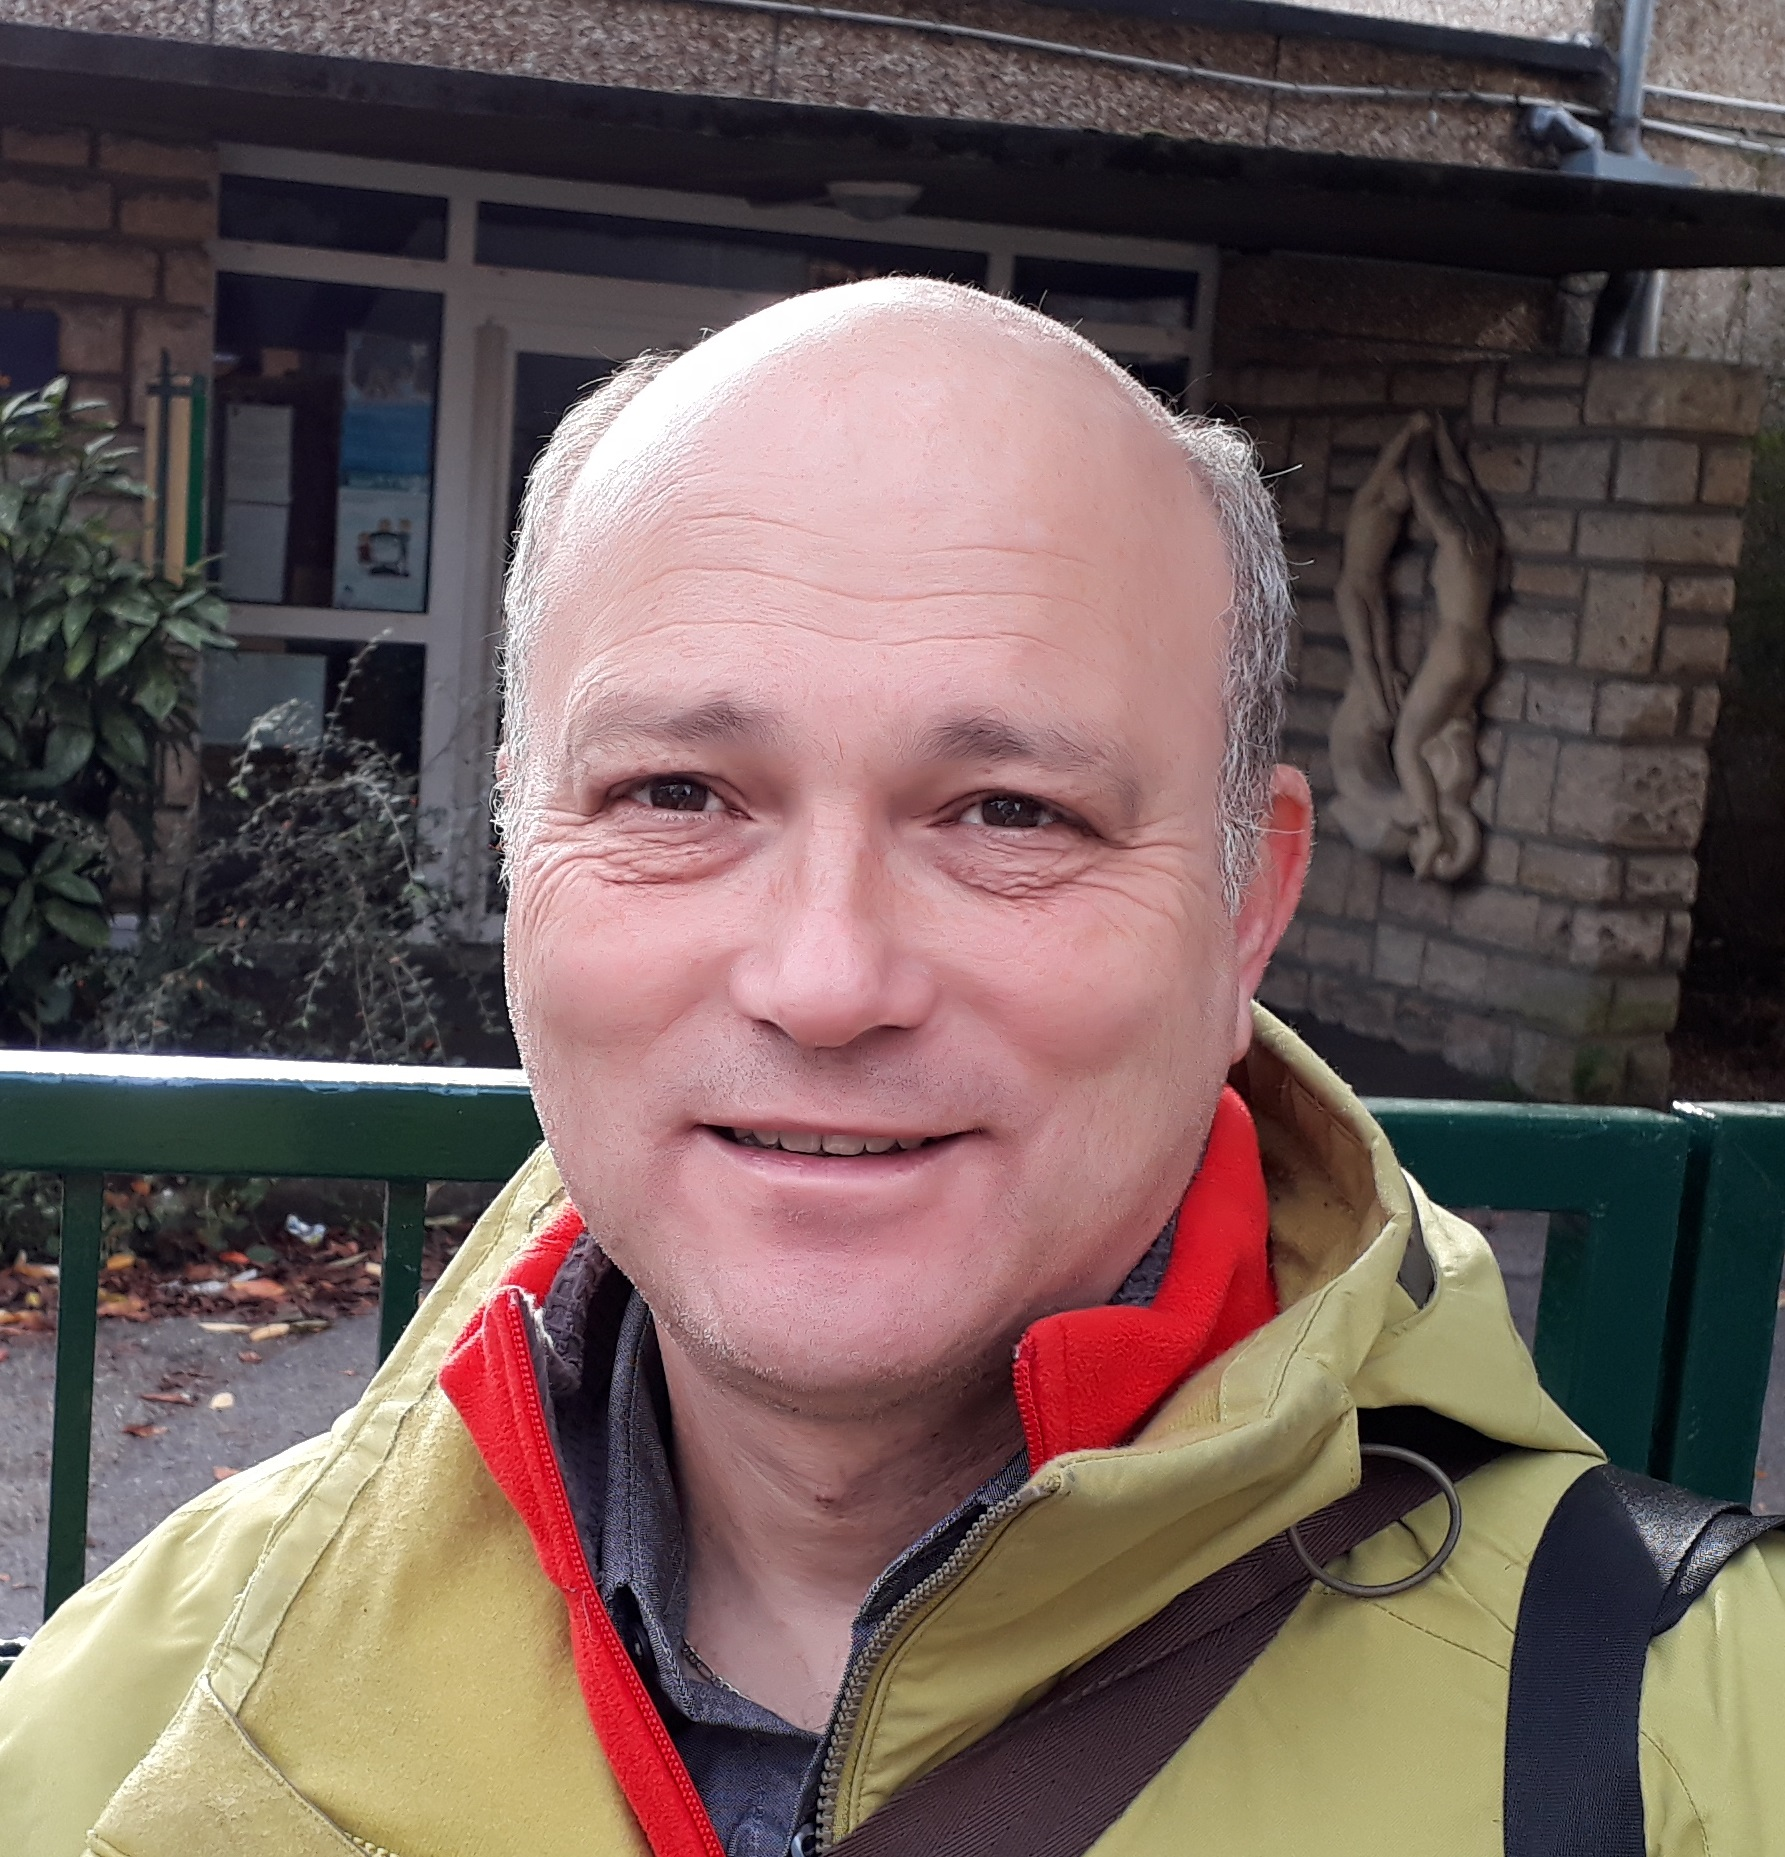
\includegraphics[width=3cm]{id.jpg}
\begin{picture}(0,0)
\setlength{\unitlength}{1cm}
%\put(-0.2,-1.5){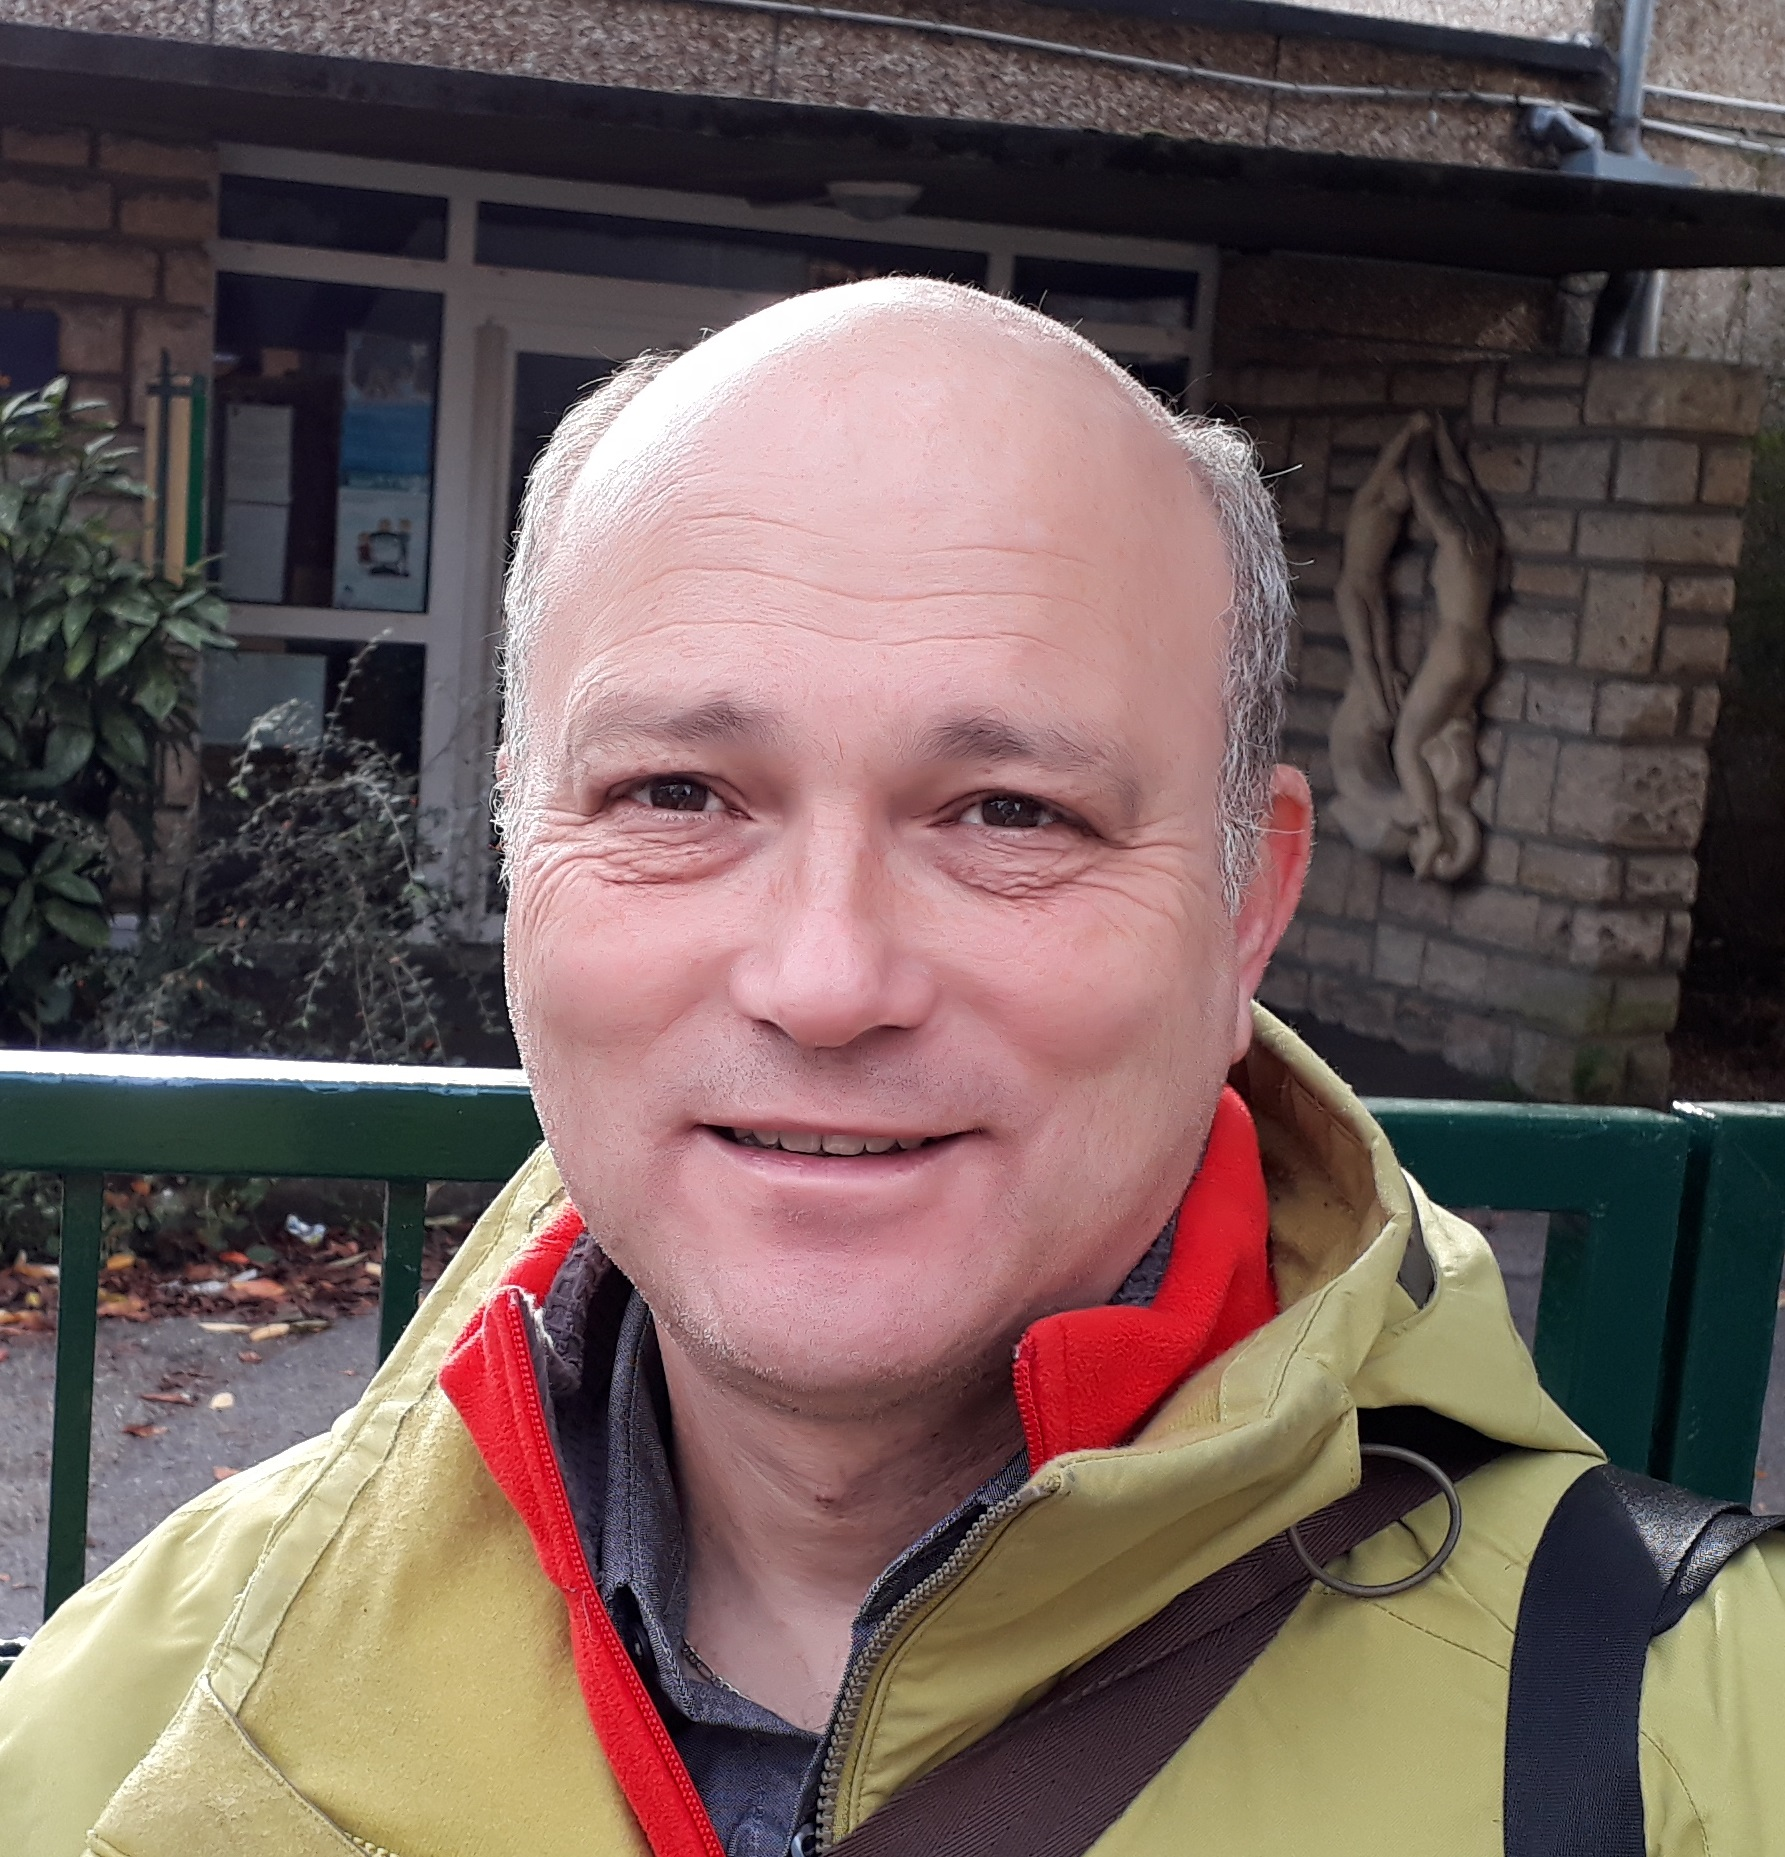
\includegraphics[scale=0.05]{id.jpg}}
\end{picture}
\makehead

%\makecvtitle

%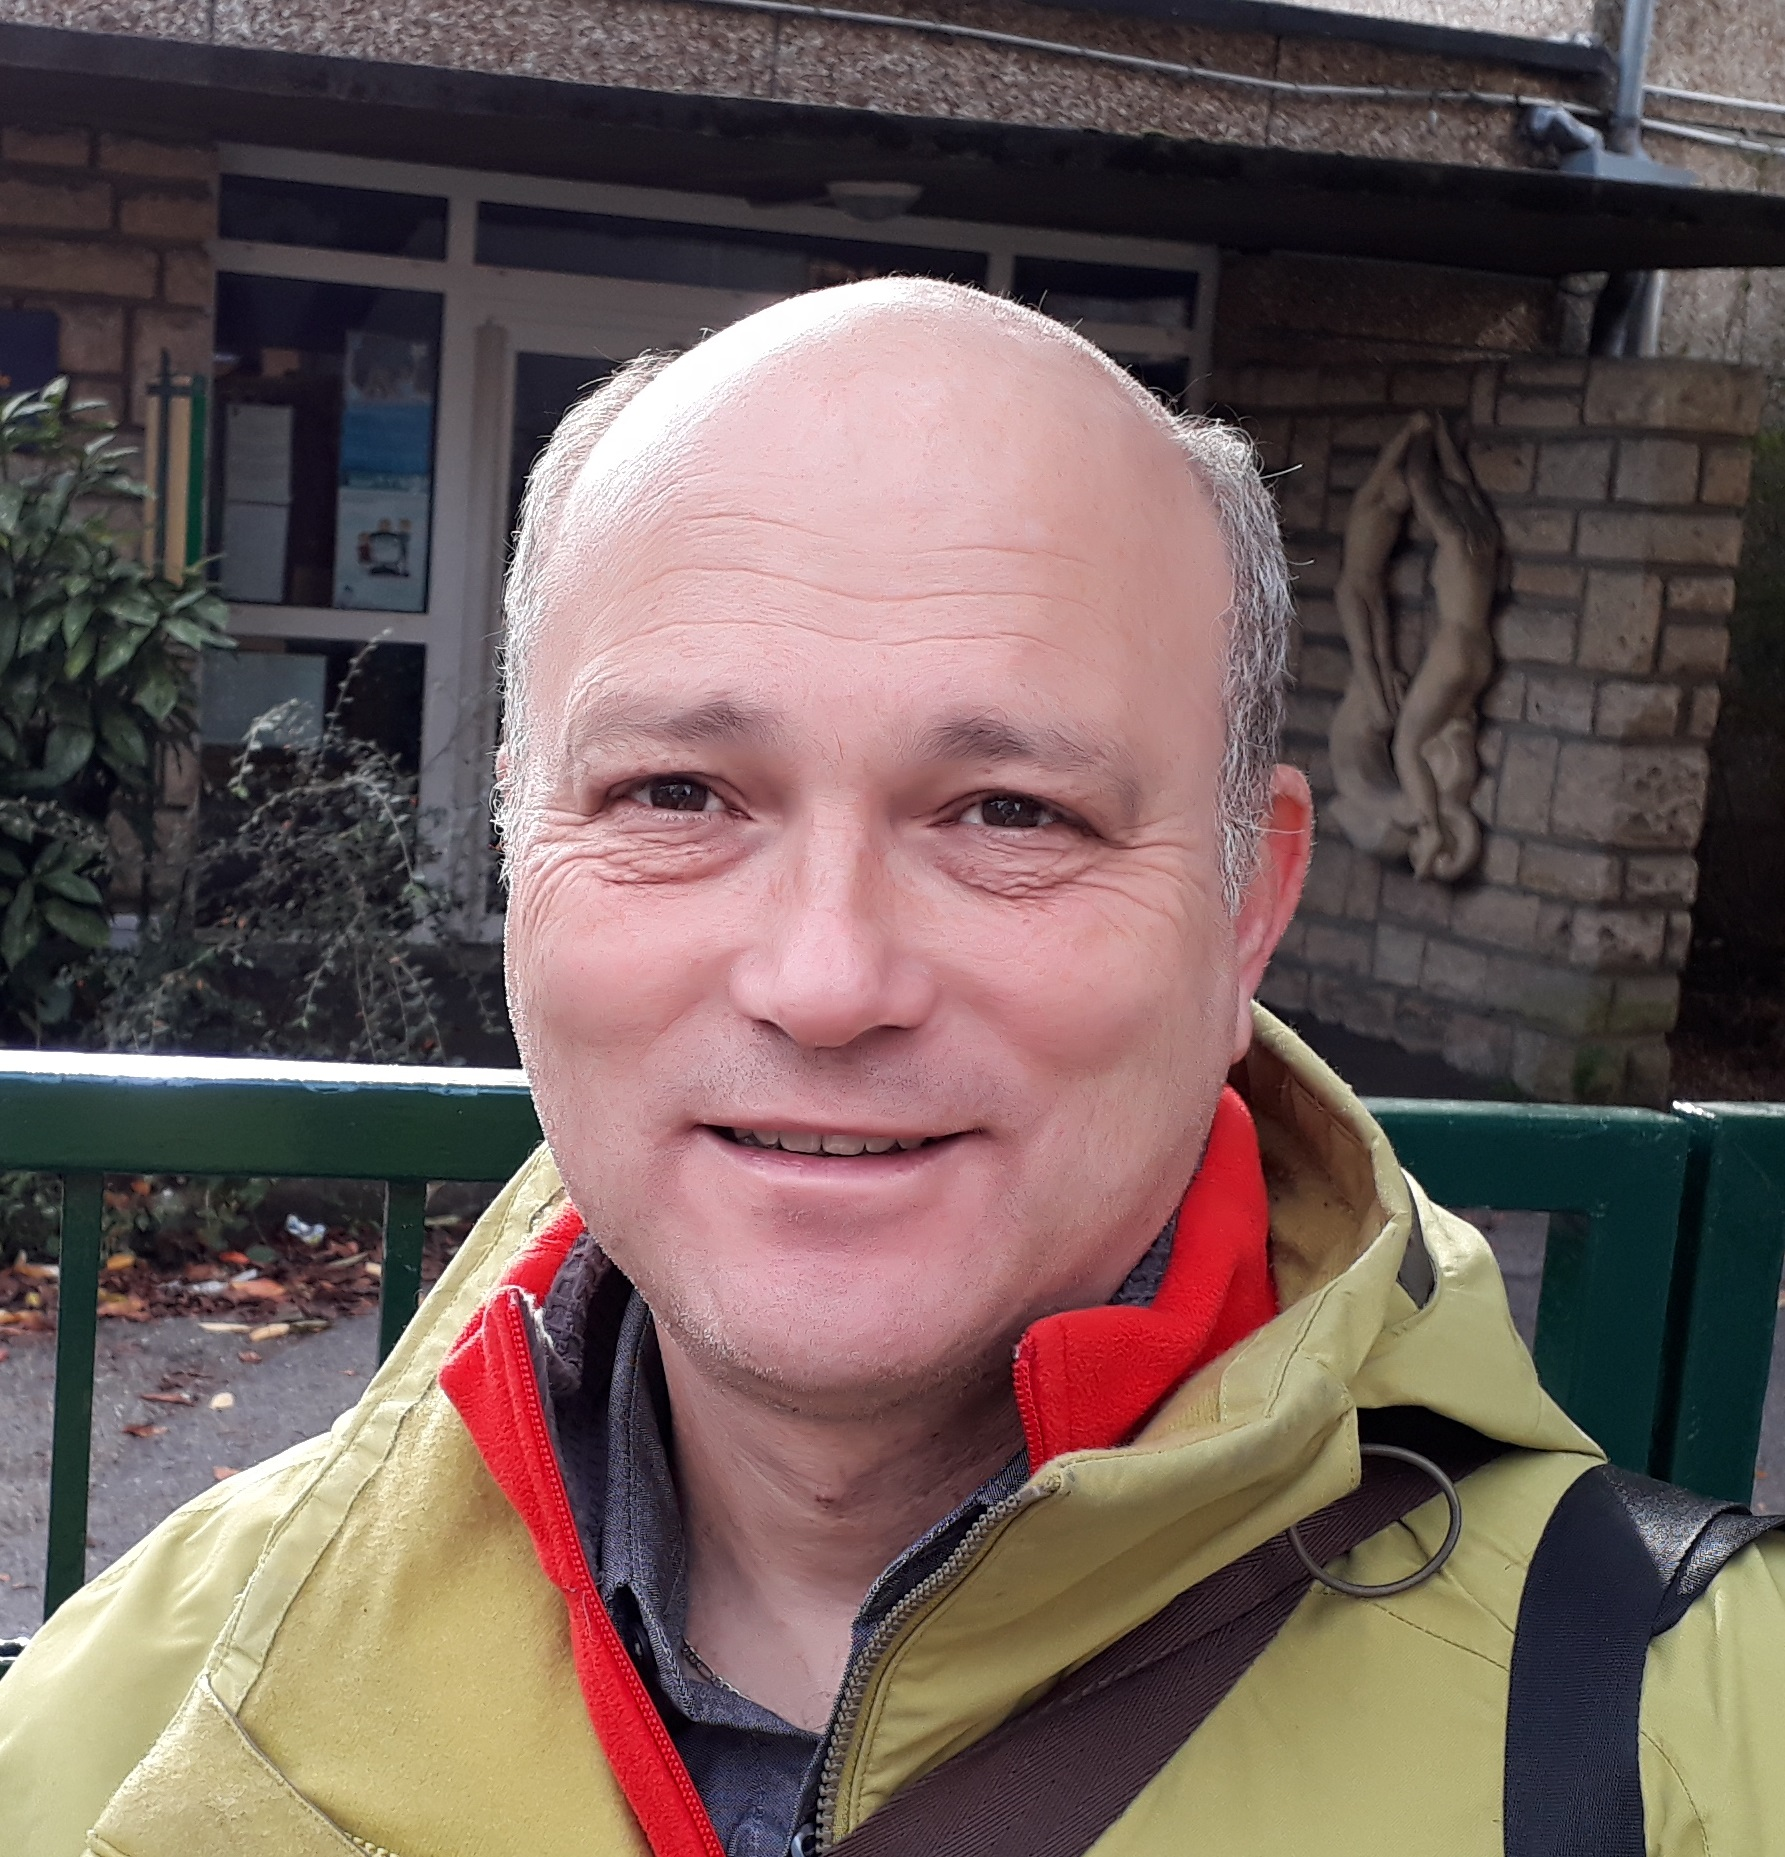
\includegraphics[width=1cm]{id.jpg}

%\small{Undergraduate electrical and electronic engineer completing the final year of a master's degree. Passionate about science, with strong technical, business, and interpersonal skills for working in a team and successfully completing a project.}

%\small{ingénieur diplômé,}
%\begin{spacing}{1.2}
\section{Formation}

%\vspace{5pt}

%\subsection{Academic Qualifications}

%\vspace{5pt}

\begin{itemize}

\item{\cventry
%{1990}
{}
{diplôme d'ingénieur de l'école Centrale }
{Ecole Centrale de Lille}
{Lille, France}
{\textit{option automatique}}
{}
}

\item{\cventry
%{1981-1984}
{}
{lycée Jacques Decour}
{Mathématiques supérieures, mathématiques spéciales}
{Paris, France}
{\textit{option M}}
{}
}




\end{itemize}

\vspace{2pt}


%----------------------------------------------------------------------------------------
%	SECTION TITLE
%----------------------------------------------------------------------------------------

\section{Expérience}

%----------------------------------------------------------------------------------------
%	SECTION CONTENT
%----------------------------------------------------------------------------------------

\begin{itemize}

%------------------------------------------------
\item{
\cventrylc
{Juin 2017 - aujourd'hui} % Date(s)
{Senior Software Architect} % Job title
{Thales Training et Simulation} % Organization
{Cergy, France} % Location
{}
{ % Description(s) of tasks/responsibilities
\\[6pt]
Cette dernière année j'ai travaillé à améliorer l'outil de production de bases de données visuelles. Cet outil permet de générer des fichiers
(base de données) utilisables au runtime par le moteur de rendu graphique, à partir d'images, de descriptions et de base de données open sources
telles que OpenStreetMap.
\\[6pt]
\begin{itemize}
\item {Architecture logicielle de ré-ingéniérie des fabrications de base de données visuelles des simulateurs.}
\item {Réduction des temps de production de plusieurs jours à quelques dizaines de minutes.}
\item {C++11, QGIS, OpenStreetMap, Collada}
\end{itemize}
}
{
}
}
%------------------------------------------------    
\item{
\cventrylc
{Septembre 2015 - Juin 2017} % Date(s)
{Senior Software Architect} % Job title
{Thales Training et Simulation} % Organization
{Cergy, France} % Location
{}
{ % Description(s) of tasks/responsibilities
\begin{itemize}
\item {Maintenance des modèles de simulation de la boucle de vol}
\item {Réécriture et encapsulation Maintenance des modèles de simulation de la boucle de vol}
\item {Matlab, Simulink, C++, Python}
\end{itemize}
}
}

%\vspace{3pt}
%\pagebreak
%------------------------------------------------
\item{
\cventrylc
{février 2004 - 2015} % Date(s)
{Senior Software Architect} % Job title
{Thales Training \& Simulation (TTS)} % Organization
{Cergy, France} % Location
{}
{
\iftoggle{anglais}
{
Within TTS I brought my experience and technical expertise at the rewriting of the simulation framework. I also drove the implementation works, and took part to the system specification
with our european partners. I was responsible of this framework, from the design to ghe support and maintainance :
\begin{itemize}
\item {System design in a european partnership for the NH90 Airbus helicopters.}
\item {Technical interface in english with our partners}
\item {Design, Implementation, Maintenance of real time framework provided by Thales}
\end{itemize}

Responsible fo the software product "framework", software cradle of the simulation models, allowing to reproduce the real time behavior of the helicopter, in order to train the pilots.
\begin{itemize}
\item{Management of a 7 engineers team.}
\item{Code generation tools allowing to generate the applicative modules interfaces, from the the UML IRS of the system. Deployment and tooling (runtime management of real time data) generation.}
\item{Deployment of TACTIS (dutch army), NH90 Helicopter (german, swiss, australian army), EC145 helicopter (french army)}
\item{Technical architecture workgroup on the NH90 program, in a difficult context with our partners/competitors from Germany, UK, Canada, France}
\item{Peer review and code quality audit}
\item{Code generators and deployment tool in python, interface database in postgres}
\item{Continuous integration, automatic asynchronous test tools in a functional programming environment (Ocaml, Erlang, AutoIT, ThalesControl (Jenkins)).}
\item{MCO (Maintien en Conditions Opérationnelles)}
\end{itemize}
}
{
Chez TTS j'ai apporté mon expérience et mon expertise technique à la refonte du framework de simulation. J'ai également assuré la conduite des travaux, de la spécification avec des partenaires européens, en passant à la réalisation, et jusqu'à la recette et à la maintenance en conditions opérationnelles :
\begin{itemize}
\item {Ingéniérie en partenariat européen pour les simulateurs NH90.}
\item {Interface technique en anglais avec les partenaires}
\item {Conception, Implémentation, Maintenance des frameworks temps réel des simulateurs réalisés par Thales}
\end{itemize}

Responsable du composant "framework", base logicielle hébergeant les modèles de simulation, permettant la reproduction du comportement temps réel de l'hélicoptère, dans le but de formation des pilotes.
\begin{itemize}
\item{	Encadrement d’une équipe de 7 ingénieurs.}
\item{	Outillage de génération du code des interfaces composant, à partir des IRS UML du système. Génération du déploiement et de l’instrumentation.}
\item{Déploiement sur les programmes TACTIS (armée de terre néerlandaise), Hélicoptère NH90 (armée de l’air allemande, suisse, australienne), hélicoptère EC145 (armée française)}
\item{Groupe de travail d’architecture technique sur le simulateur d’hélicoptère NH90, dans un contexte difficile avec nos partenaires/compétiteurs allemands, anglais, canadiens, français (qui sont nos concurrents sur d’autres affaires).}
\item {Conduite de revue de pairs et audit de qualité du code}
\item {Mise en place d’un environnement de d’intégration continue (tests automatiques) dans un environnement de programmation fonctionnelle (Ocaml, Erlang, AutoIT, ThalesControl (Jenkins)).}
\item {MCO (Maintien en Conditions Opérationnelles)}
\end{itemize}
}

}
} %item

%\pagebreak
%------------------------------------------------
\item{
\cventrylc
{Novembre 1998 - février 2004} % Date(s)
{Senior Software Architect} % Job title
{Thales Raytheon Systems (TRS)} % Organization
{Massy, France} % Location
{}
{ % Description(s) of tasks/responsibilities
Au sein de TRS j'étais responsable de la conception, l'implémentation, la maintenance et le support des frameworks logiciels des centres de contrôles aérien militaires. Les caractéristiques prépondérantes de ce framework sont~:
\begin{itemize}
\item{fiabilité : le framework apporte des services de reconfiguration, persistence et communication pour que le système soit disponible 24/24, même en cas de panne (par exemple, crash d'un applicatif) }
\item{variabilité : le framework est déployé sur différents systèmes (France, OTAN, Suisse, ...), qui ont des spécifications différentes}
\item{simplicité : le framework est utilisé par des partenaires et des sous-traitants multiples. Sa simplicité de mise en oeuvre, l'API limitée à quelques fonctions, le reporting sont un gage du succès du système global.}
\item{chiffres : 100K lignes de code C++, encadrement d'une équipe de 8 personnes. Maintenance sur plusieurs dizaines d'années.}
\end{itemize}
\myvspace
Le framework étant l'interface technique des composants applicatifs, j'ai également eu des travaux de~:
\begin{itemize}
\item {Ingéniérie en partenariat européen (NATO) et USA (Raytheon) sur le projet NATO LOC1 (contrôle aérien militaire de l'OTAN)}
\item {Interface technique en anglais avec le partenaire Raytheon}
\end{itemize}
\myvspace
Le framework a été déployé sur les autres systèmes de contrôle aérien livrés par TRS, avec une technique d'approche de variabilité, permettant de minimiser les variations dans l'implémentation du produit par rapport aux différences importantes dans les exigences client.
 \begin{itemize}
 \item SEROS (contrôle aérien militaire de la Belgique, installé à Semmerzake)
 \item Florako (Suisse)
 \item CLM (France, intégration à Mont de Marsan)
 \item ACCS LOC1 (Contrôle aérien des forces de l'OTAN)
 \end{itemize}
}
\vspace{3pt}
}

%------------------------------------------------
\itemexperience{
\cventrylc
{octobre 1990 - novembre 1998} % Date(s)
{Ingénieur R~\&~D } % Job title
{ADERSA (société de recherche sous contrat)} % Organization
{Massy} % Location
{
}
{ 
% Description(s) of tasks/responsibilities
(web : \href{https://www.sherpa-eng.com/}{https://www.sherpa-eng.com/})
\iftoggle{anglais}
{Study of non linear systems and control synthesis.
In this small company of 40 engineers, I was responsible of the design, implementation, support and takings of non-linear control software. The object was the study of a complex physical system, for instance the angle of list of an aircraft carrier during a gyration, and then create matlab model of the system, with either physical differential equations or transfert functions.
}
{
Etude de systèmes non linéaires et synthèse d'asservissements.
Au sein de cette PME de 40 ingénieurs, j'étais responsable de la conception, implémentation, support et recette de lois de commande non linéaire. Il s'agissait d'étudier un problème physique complexe, comme par exemple la gite d'un porte-avion lors de la giration, de le modéliser sous matlab sous forme d'équations physiques, ou d'identifier des fonctions de transfert.
}
\newline
\iftoggle{anglais}
{
The identification is done with data science toolboxes, provided by the Matlab ecosystem.
The job was then to synthesize a control law, allowing to control the system, as required by the client specifications, as for instance to keep the ship deck horizontal during the gyration.
}
{
L'identification se faisait à l'aide d'outils de data science, fournis par des librairies de l'écosystème Matlab.
 Il fallait ensuite synthétiser une loi de commande permettant d'asservir le système pour lui faire respecter le besoin du client, comme par exemple garder le pont du porte-avions à plat lors de la giration du batiment.
}
\newline
\iftoggle{anglais}
{
Examples of projets :
\begin{itemize}
\item {for the french DCN : control of list angle under gyration of the Charles de Gaulle aircraft carrier}
\item {for the DDE 94 : control of sewage water flows for the Valenton wastewater treatment plant}
\item {for Béghin-Say : control of sugar crystallization of the Abbeville sugar plant}
\item {technologies : Matlab/Simulink, C, C++}
}
{
Exemples de projets :
\begin{itemize}
\item {pour la DCN : contrôle de gite sous giration du porte avions Charles de Gaulle}
\item {pour la DDE 94 : contrôle des débits d'eau usée pour la station d'épuration de Valenton}
\item {pour Béghin-Say : contrôle de la cristallisation du sucre de l'usine d'Abbeville}
\item {technologies : Matlab/Simulink, C, C++}
}
\end{itemize}
%\small{
%\newline
\iftoggle{anglais}{
For some projects the control law was written in C, tested under matlab and implanted in the system, thus leading to a qualification campaign, support and maintenance.
}
{
Pour certains systèmes la loi d'asservissement était implémentée en C, testée sous matlab et implantée dans le système, ce qui impliquait une campagne de qualification et la maintenance en production.
}
%}
} %bloc cventry
} %item
\end{itemize}
%\newpage
\section{Compétences}

\begin{itemize}

\myitem
{Méthodes :}{agile, UML, SADT}

\myitem
{Languages :}{C, C++11, C++, STL, templates, Python, OCaml, OMake, CMake, Matlab/Simulink, LaTeX, Rugy, Java, Erlang, sql, Xml, Json, Corba, multithreading}

\myitem
{Outils :}{git, clearcase, Jenkins, cmake, ctest, emacs, visual studio, wix, jenkins, jira, modelers UML, eclipse, maven, matlab toolboxes (data science, identification toolbox, robust control)}

\myitem
{architecture :}{systèmes logiciels complexes, temps réel(simulateur hélico), disponibilité 24/24 (contrôle aérien), sans interruption de service}

\myitem
{OS :}{Linux, Unix (HP-UX, Solaris), Windows}

\myitem
{Cloud} : {AWS}

\myitem 
{Web :}{Apache, Ruby on Rails, javascript, JQuery}

\myitem 
{Database:}{Postgres, sql}

\end{itemize}

\iftoggle{anglais}
{
\section{Languages}
\begin{itemize}
\itemskill
{French :}
{Mother tongue}
\itemskill
{English :}
{Fluent. American spouse. Software architecture in NATO context. End of studies internship in UMIST (Manchester)
}
\itemskill
{German :}
{Fluent. 7 years student in Goethe Institut Paris, ZMP degree (Zentrale Mittelstuffenprüfung) }
\end{itemize}
}
{
\section{Langues}
\begin{itemize}
\itemskill
{Français :}
{Langue maternelle}
\myitem
{Anglais :}
{Courant. Epouse américaine. Travaux d'ingéniérie dans des contextes NATO. Stage de fin d'études à UMIST (Manchester)
}
\itemskill
{Allemand :}
{Courant. 7 ans au Goethe Institut Paris, diplôme du ZMP (Zentrale Mittelstuffenprüfung) }
\end{itemize}
}
%----------------------------------------------------------------------------------------
%	SECTION TITLE
%----------------------------------------------------------------------------------------

\iftoggle{anglais}
{
\section{Other occupations}
\small{
Trekking : Ethiopie (Siemen), Tanzanie (ascent of Kilimandjaro, Zanzibar), Himalaya (Ladakh,Zanskar) 
\newline
Orienteering races : active member of a club (runner, management of software in competitions)
\newline
Marathon : Paris 2013, 2015, 2016, 2019?
\newline
Musique : lead guitar in an rock band, amateur concerts
}
}
{
\section{Autres activités}
\small{
Trekking : Ethiopie (Siemen), Tanzanie (ascension du Kilimandjaro, Zanzibar), Himalaya (Ladakh,Zanskar) 
\newline
Course d'orientation : membre actif d'un club (coureur, gestion informatique des compétitions)
\newline
Marathon : Paris 2013, 2015, 2016, 2019?
\newline
Musique : guitariste lead d'une formation rock, concerts amateur
}
}

%------------------------------------------------

\vspace{3pt}

%\small{This challenging project took place over the entirety of my third year. It required excellent planning and organisational skills, and the ability to teach myself an entirely new and complex subject. The project was a success, with the system being able to localise a radioactive source down to $ 3 cm$ within a $ 600 m^3$ sensor array. This project has been suggested for publication by my supervisor.}

%\vspace{6pt}
%%\section{Interests and extra-curricular activity}

\vspace{6pt}

\begin{itemize}

\item{I was a "fresher representative" in my 2nd and 3rd years of university, this required me to guide, look after, and ensure that a particular flat of first years have a good time in their first week, and feel consoled in what for most of them is there first time living away from home. We were responsible for the safety and wellbeing of the group of first years during the first week, and during this time I made good friends with all of them.}

\vspace{6pt}

\item{I am a member of a number of university societies. I was also the vice president and co-founder of the flash mob society. My roles in this included recruiting members, in which during "fresher's fair" we enlisted over 200 new members. This was regarded as very successful, considering other societies averaged around 50. I also appeared in an interview on the university television station, set up a society bank account, and helped organise the events. One of these events was featured in the local newspaper.}

\vspace{6pt}

\item{I am also an avid hiker, having completed the national 3 peaks challenge last summer. Other interest include guitar, which I am self-taught, and home brewing.}

\end{itemize}



\iftoggle{anglais}
{
\section{References}
\vspace{6pt}
\begin{itemize}
\item{available on request}
%\item{disponibles sur demande}
\end{itemize}
}
{
\section{Références}
\vspace{6pt}
\begin{itemize}
%\item{available on request}
\item{disponibles sur demande}
\end{itemize}
}


%\end{spacing}
% Publications from a BibTeX file without multibib
%  for numerical labels: \renewcommand{\bibliographyitemlabel}{\@biblabel{\arabic{enumiv}}}% CONSIDER MERGING WITH PREAMBLE PART
%  to redefine the heading string ("Publications"): \renewcommand{\refname}{Articles}
%\nocite{*}
%\bibliographystyle{plain}
%\bibliography{publications}                        % 'publications' is the name of a BibTeX file

% Publications from a BibTeX file using the multibib package
%\section{Publications}
%\nocitebook{book1,book2}
%\bibliographystylebook{plain}
%\bibliographybook{publications}                   % 'publications' is the name of a BibTeX file
%\nocitemisc{misc1,misc2,misc3}
%\bibliographystylemisc{plain}
%\bibliographymisc{publications}                   % 'publications' is the name of a BibTeX file

%-----       letter       ---------------------------------------------------------

\end{document}


%% end of file `template.tex'.
